\section{Filtre}
This project utilizes two types of filter a FIR (finite inpulse responds) 
filter and an IIR (infinite impulse responds) filter.
The FIR filter is designed and implemented in matlab using the window method.

\subsection{FIR Filter Design}
First step in designing a FIR filter is to design an ideal IIR filter before
trucating it with by multiplying the IIR filter with a finite length window
function. 

By using our spectral analysis from the earlier sections, we qualitatively
decided to make the cutoff frequence $f_{c} = 10$. The sample frequency $f_{s}$
is given from our dataset, $f_{s} = 47.7774$.

Lastly, the filters made order $M = 250$ thus using $250$ filter coefficients. 

\subsubsection{Resolution}
Next step in designing our filter, we determine the frequency resolution
which provides specifications for the FIR transfer function.

\begin{align}
  \label{eq:freqResolution}
  f_{res} &= \frac{f_{s}}{M}
\end{align}

\subsubsection{Transfer function}
Using $f_{res}$ and $f_{c}$, we can determine which frequency bin
corresponds to frequencies below $f_c$.
This must be in done in integer values i.e.\ rounded to 
closes integer value.

\begin{align}
  \label{eq:freqBin}
  f_{bin} = \left\lfloor\frac{f_{c}}{f_{res}}\right\rfloor = 52
\end{align}

In this case the bin number corresponds to $f_c$ is 52, which
we design our lowpass filter around see \autoref{fig:specificatiion}.

These specification help determine which frequencies should be passed and which should be removed. In this case we remove everything above frequency 10.

\begin{figure}[h]
  \centering
  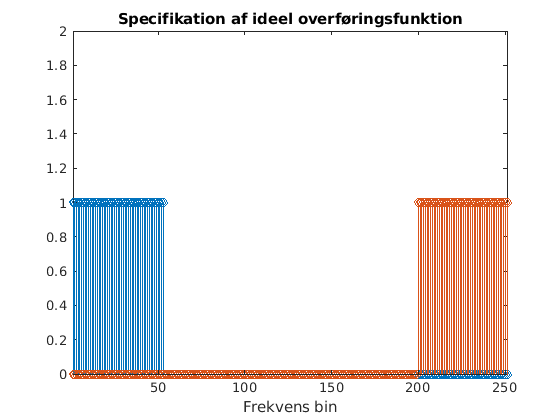
\includegraphics[scale = 0.5]{matlabStuff/Specification_of_transfer_function.png}
  \caption{Specification for our transfor function}%
  \label{fig:specificatiion}
\end{figure}

\newpage

In matlab we can now make our transfer function $h$ using the follwing code. Which when combined with, in our case a hanning window function serves to become our filter which we can run our
data set through.

\begin{figure}[h]
  \centering
  \lstinputlisting[language={matlab}, linerange={27-28,40-40,49-50,58-60}]{matlabStuff/filter.m}
  \caption{matlab code for making a transfer function}%
  \label{}
\end{figure}

Now that we have our transfer function, we can apply it to our data to see if we can reduce the potential noice in data.\
we can plot its coefficients together with the window function, along with the resultat transfer function to see if it
does indeed ``cover'' the peak around $10Hz$.

\begin{figure}[h]
  \centering
  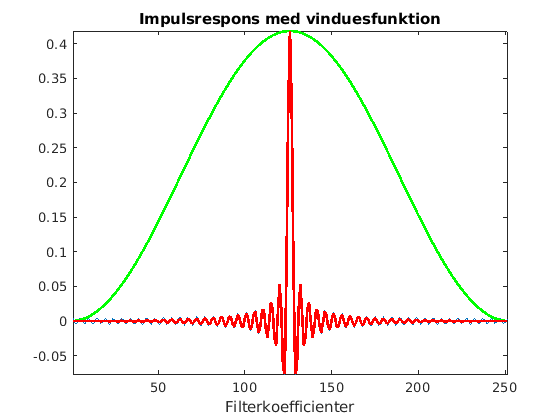
\includegraphics[scale=0.75]{matlabStuff/impulsresponds_with_window.png}
  \caption{Impulseresponds overlayed with the window function, showing its koefficent values as functions of index numbers}%
  \label{fig:impulserespondsWithWindow}
\end{figure}

\newpage

\begin{figure}[h]
  \centering
  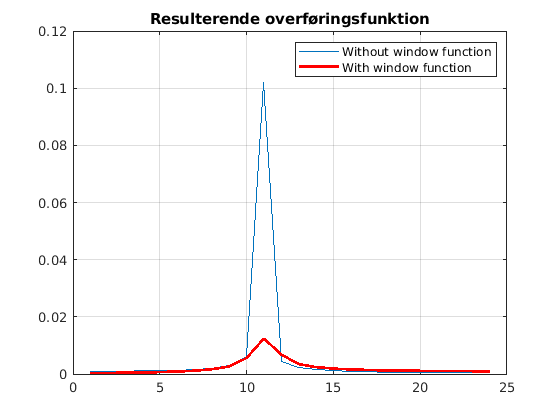
\includegraphics[scale=0.65]{matlabStuff/resuting_transfer_function.png}
  \caption{Resulting transfer function overlayed with and without the window function}%
  \label{fig:resultingTransferFuntion}
\end{figure}

\subsubsection{Applying the FIR filter}
With all of the preperation work done, we can now apply our filter to our dataset to see the results.

\begin{figure}[h]
  \centering
  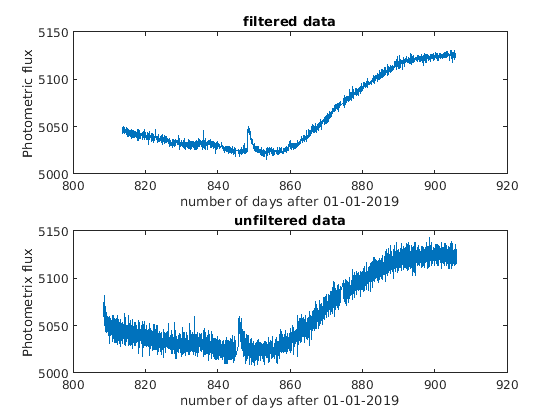
\includegraphics[scale=0.62]{matlabStuff/datasetComparison.png}
  \caption{Side by side comparison of the data before and after the filter has been applied}%
  \label{fig:datasetComparison}
\end{figure}

Its clear fron this comparison that we have manage to remove a some of the signal noice, but since this data set does not show
anything usefull (the spike is a kalibration issue), we wont be able to tell anything from this filtering.

\newpage

\subsection{IIR Filter}

For the IIR filter the ``butter'' function has been used
too design the transfer function and thus produce the 
filtering coefficients.

Once this has been done everything plays out much like the 
FIR filter, we can plot our transfer function and the 
hanning window function to see the coefficients
and their values as functions of indexing.

\begin{figure}[h]
  \centering
  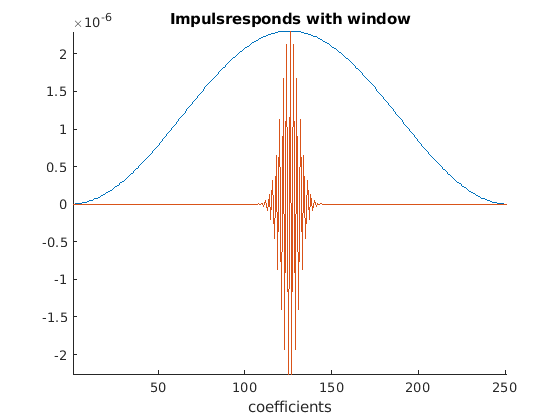
\includegraphics[scale=0.60]{matlabStuff/IIR_responds_with_window.png}
  \caption{Impulse responds with window function for the IIR filter}%
  \label{fig:resultingTransferFuntionIIR}
\end{figure}

Here we can see that the new Impulseresponds does not 
tapper at all compared to the FIR filter which did 
tapper off toward the center.

\begin{figure}[h]
  \centering
  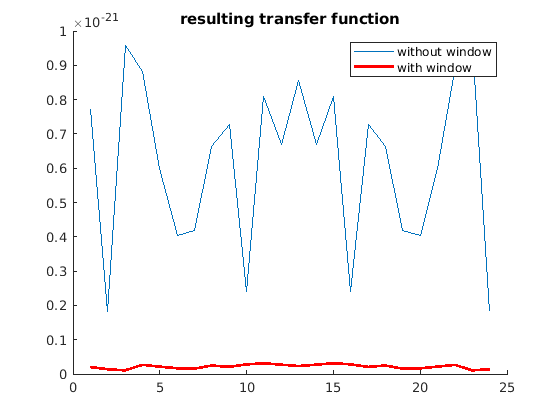
\includegraphics[scale=0.60]{matlabStuff/resulting_filter_function_IIR.png}
  \caption{Resulting transfer function overlayed with and without the window function}%
  \label{fig:resultingTransferFuntionIIR}
\end{figure}

unlike the FIR filter which produce a simple peak, and reduced peak for our transfer function the IIR butterfilter, has
produced a resulting transfer function that seem to cover the entire spectre of frequencies.

Note also that when the window function is applied to it, it is
substantially reduced, over the entire spectre as well.

Finally lets see what the result off applying this filter to our original data.

\begin{figure}[h]
  \centering
  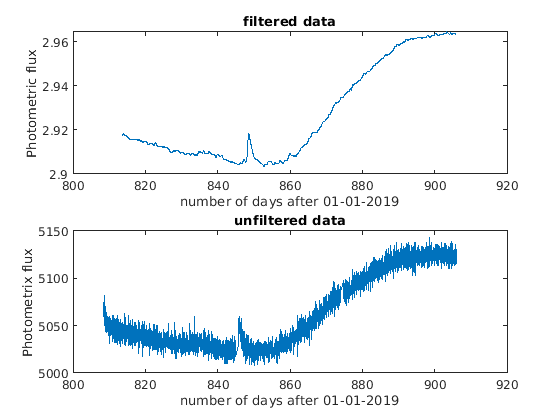
\includegraphics[scale=0.60]{matlabStuff/IIRFilterCompare.png}
  \caption{Data comparison for original data and IIR filtered data}%
  \label{fig:IIRCompare}
\end{figure}

As we can see in \autoref{fig:IIRCompare} this has removed any
hint of noice, but if there were significant data in this
dataset it might have remove that as well.
IIR could therefore at least in this case be too strict of a 
filter to use and the FIR filter might therefore be prefered.

\newpage

\subsection{Experimenting with different cutoff frequencies and orders}
If we try with a different cutoff frequency, compared to what
was seen in \autoref{fig:datasetComparison} we can see that
lowering the frequency cutoff for our lowpass filter
means that we are removing more potential noice, but
also have a higher chance of removing vital data points.

\begin{figure}[h]
  \centering
  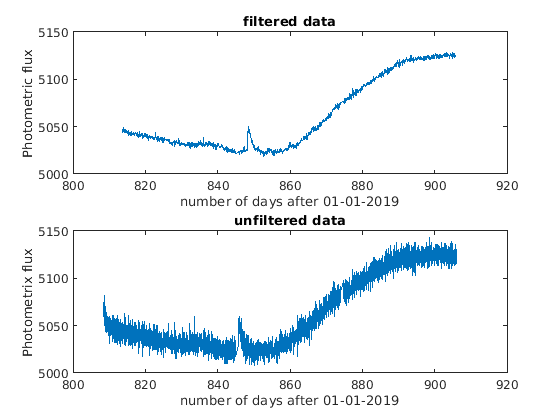
\includegraphics[scale=0.60]{matlabStuff/FIR20CutOff.png}
  \caption{Data comparison for original data and $f_{c}=5$ instead of the origianl $f_c = 10$}%
  \label{fig:resultingTransferFuntion20cutoff}
\end{figure}

Its not shown here but not that it will in general lead to a
wider Impulseresponds and vice versa for higher frequence cutoffs.

\begin{figure}[h]
  \centering
  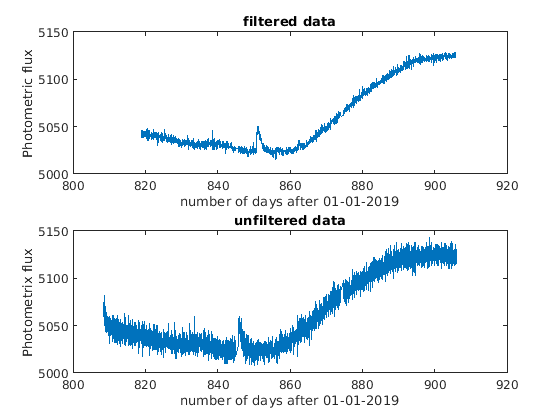
\includegraphics[scale=0.60]{matlabStuff/datasetHigherOrder.png}
  \caption{Data comparison for original data and higher order filtered data}%
  \label{fig:resultingTransferFuntion20cutoff}
\end{figure}

Here we dont see much difference, maybe because the filter order is alread very high, but we can see that the data is a little more refined that for \autoref{fig:datasetComparison}.
Obviously if we had a lower order filter the data would be less refined once filtered.



\newpage

